\chapter{システム仕様書章立て生成プロンプト}\label{cha:Proposal}

本章では、本研究で提案するシステム仕様書章立て生成プロンプトについて述べる。

\section{プロンプトの利用手順}
\label{sec:process}

提案するシステム仕様書章立て生成プロンプトの利用手順は、以下の2ステップである。
また、提案するシステム仕様書章立て生成プロンプトの構成を、図\ref{fig:prompt_structure}に示す。
以降、提案するシステム仕様書章立て生成プロンプトを「提案プロンプト」とする。

\begin{figure}[tp]
  \centering
  \includegraphics[width=0.9\linewidth]{images/prompt_figure.pdf}
  \caption{提案プロンプトの構成}
  \label{fig:prompt_structure}
\end{figure}

\begin{enumerate}
    \item \textbf{システム情報の入力}:
    ユーザー(仕様書作成者)は、図\ref{fig:prompt_structure}の「開発するシステム情報」部分に、対象システムのシステム名とシステム概要を記述する。

    \item \textbf{章立ての生成}:
    章立て生成の対象とする「開発するシステム情報」を入力したプロンプトをLLM(GPT-5.2)に入力し、システム仕様書の章立てを生成する。出力結果として、章立て(章・節・項の構造)を得る。
\end{enumerate}


\section{プロンプトの構成}

提案プロンプトの作成には、Jules Whiteらによるプロンプトパターンカタログ\cite{prompt-patterns}を参考にする。
提案プロンプトは、以下の5つの要素で構成する(図\ref{fig:prompt_structure}を参照)。
\begin{itemize}
  \item 役割付与
  \item ベースの章立て  
  \item 開発するシステム情報
  \item システム仕様書の定義
  \item 章立て出力指示
\end{itemize}

提案プロンプトのテンプレートを、図\ref{fig:prompt_full_text}に示す。

\begin{figure}[tp]
\begin{tcolorbox}[
  colback=white,
  colframe=blue,
  fonttitle=\bfseries,
]
\footnotesize
\ttfamily
\fontsize{7}{7}\selectfont
\begin{verbatim}
あなたはシステム仕様書作成の専門アシスタントです。

【ベース章立てテンプレート(参考)】
1. 概要
 1.1.目的
 1.2.システム概要
 1.3.適用範囲
2. システム基本条件
 2.1.稼働条件
 2.2.他システムインターフェース
 2.3.性能条件
 2.4.拡張条件
 2.5.継承条件
 2.6.以降環境
3. システム構成
 3.1.ハードウェア構成及びネットワーク構成
 3.2.ソフトウェア構成
4. システムの機能
 4.1.機能構成
 4.2.個別機能概要
5. システムの運用
 5.1.運用方法
 5.2.各業務(機能)の運用
 5.3.障害時の運用
6.セキュリティ
7.安全設計
8.データ仕様
 8.1.コード体系
 8.2.データベース
 8.3.ファイル
 8.4.入出力データ
 8.5.メッセージ
9.付帯事項

※ベース章立てはあくまで参考です。必要に応じて章の追加・削除・順序変更を行って、漏れなく体系的な章立てを作成してください。

【開発するシステム情報】
- システム名：
- 概要：

【システム仕様書の定義】
- 目的：
 ・プログラム作成者がシステムの仕様を理解し、設計・実装するための文書 
 ・システムテスト担当者がテスト項目を作るために参照する文書
- 対象読者:
 ・プログラム作成者：新人想定 
 ・テスト担当者：内部構造は知らず、仕様書に記載されたエラー条件に従ってテストを実施
- 記述スタイル：
 ・専門用語は必ず説明 
 ・初出の単語は必ず説明 
 ・システム概要は図を使って視覚的に理解できるようにする 
 ・図はユースケース図または独自の簡易図を使用し、必ずテキストで補足説明 
 ・用語や機能名は文書内で統一 
 ・データ型や制約が必要な場合は表形式で記載 
 ・外部仕様のみ記載(内部構造は書かない)
- システム要件：
 ・動作環境：OS、ハードウェア、ネットワーク 
 ・非機能要件：パフォーマンス、セキュリティ 
- 記述の粒度：
 ・画面レイアウトと操作フローのみ含める

【出力指示】
・上記情報に基づき、開発するシステムのシステム仕様書に必要な章立てを出力してください。
・ここでいう章立ては、以下の内容を含みます。
　・章と節、章タイトル、節タイトル、項、項タイトル 
・出力形式は**マークダウンの番号付きリスト**としてください。 
・章名以外(目的・記述のポイントなど)は一切書かないでください。 
・章の追加や削除、順序の変更は自由に行って構いません。
・人間が考慮し忘れるような章立ても考えるのがあなたの役目です。考慮漏れが無いように、網羅性を高めてください。
\end{verbatim}
\end{tcolorbox}
\par\vspace{-20pt}
\captionof{figure}{提案プロンプトのテンプレート}
\label{fig:prompt_full_text}
\end{figure}

% \subsection{プロンプト構成要素}

% 本節では、提案プロンプトを構成する5つの要素について説明する。
以降、提案プロンプトを構成する5つの要素について説明する。
表\ref{tb:prompt_elements_summary}に、各要素の役割と関連するプロンプトエンジニアリング技術(\ref{sec:prompt_engineering}節を参照)の対応を示す。

\begin{table}[tp]
  \caption{提案プロンプト構成要素と対応する技術と目的}
  \label{tb:prompt_elements_summary}
  \centering
  \small
  \begin{tabular}{|l|p{8cm}|l|} % 幅を調整
    \hline
    \textbf{構成要素} & \textbf{目的と解決する課題} & \textbf{関連技術} \\
    \hline
    役割付与 & 専門的な文体と観点の固定 & Persona Pattern \\
    \hline
    ベースの章立て & 構造の欠落防止、標準的な形式の担保 & One-shot Prompting \\
    \hline
    開発するシステム情報 & 生成内容の具体化 & Context Manager Pattern \\
    \hline
    仕様書の定義 & 記述粒度の制御、不必要な内部情報の排除 & Context Manager Pattern \\
    \hline
    章立て出力指示 & 論理的整合性の確保、出力結果の視認性の確保 & Template Pattern \\
    \hline
  \end{tabular}
\end{table}

\subsubsection{役割付与}

図\ref{fig:prompt_full_text}における「役割付与」部分のプロンプトを、図\ref{fig:role_assignment}に示す。

\begin{figure}[tp]
\vspace{9mm}
\begin{tcolorbox}[
  colback=white,
  colframe=blue,
  fonttitle=\bfseries,
]
\footnotesize
\ttfamily
\fontsize{10}{11}\selectfont
\begin{verbatim}
あなたはシステム仕様書作成の専門アシスタントです。
\end{verbatim}
\end{tcolorbox}
% \par\vspace{-20pt}
\captionof{figure}{「役割付与」部分のプロンプト}
\label{fig:role_assignment}
\end{figure}

プロンプトの文頭で「あなたはシステム仕様書作成の専門アシスタントです」と書くことで、LLMに特定の役割を与える。
これは、\ref{subsec:persona_pattern}節で述べたPersona Pattern(ペルソナパターン)の適用である。
提案プロンプトでは、「システム仕様書作成の専門アシスタント」という役割をLLMに与えることで、LLMの出力をシステム仕様書作成に適したものにする。

\subsubsection{ベースの章立て}

図\ref{fig:prompt_full_text}における「ベースの章立て」部分のプロンプトを、図\ref{fig:base_outline}に示す。
実際の開発現場で使用されている章立てのテンプレートを「ベース章立てテンプレート」として提示する。
これは、\ref{subsec:one_shot}節で述べたOne-shot Promptingの技術を用いて、出力する章立て構造の例示を行っている。



\begin{figure}[tp]
\begin{tcolorbox}[
  colback=white,
  colframe=blue,
  fonttitle=\bfseries,
]
\footnotesize
\ttfamily
\fontsize{9}{10}\selectfont
\begin{verbatim}
【ベース章立てテンプレート(参考)】
1. 概要
 1.1.目的
 1.2.システム概要
 1.3.適用範囲
2. システム基本条件
 2.1.稼働条件
 2.2.他システムインターフェース
 2.3.性能条件
 2.4.拡張条件
 2.5.継承条件
 2.6.以降環境
3. システム構成
 3.1.ハードウェア構成及びネットワーク構成
 3.2.ソフトウェア構成
4. システムの機能
 4.1.機能構成
 4.2.個別機能概要
5. システムの運用
 5.1.運用方法
 5.2.各業務(機能)の運用
 5.3.障害時の運用
6.セキュリティ
7.安全設計
8.データ仕様
 8.1.コード体系
 8.2.データベース
 8.3.ファイル
 8.4.入出力データ
 8.5.メッセージ
9.付帯事項

※ベース章立てはあくまで参考です。必要に応じて章の追加・削除・順序変更を行って、漏れなく体系的な章立てを作成してください。
\end{verbatim}
\end{tcolorbox}
\par\vspace{-20pt}
\captionof{figure}{「ベースの章立て」部分のプロンプト}
\label{fig:base_outline}
\end{figure}


LLMにテンプレートを与えず、ゼロから章立てを生成させると、章の順序が不自然になる、重要な章(例：セキュリティや運用)が抜け落ちるといった「構造的な欠陥」が生じるリスクがある。
そこで、提案プロンプトでは、実際の開発現場で用いられている章立てのテンプレートを初期値(ベース)としてLLMに与えることで、LLMは「何を書くべきか」の探索範囲を絞り込むことができる。
ベースの章立てテンプレートの提示により、章立ての標準的な構成を維持する。

\subsubsection{開発するシステム情報}

 図\ref{fig:prompt_full_text}における「開発するシステム情報」部分のプロンプトテンプレートを、図\ref{fig:development_system_info_template}に示す。
これは、本プロンプトの入力であるシステム名とシステム概要を記述する箇所である。


\begin{figure}[tp]
\begin{tcolorbox}[
  colback=white,
  colframe=blue,
  fonttitle=\bfseries,
]
\footnotesize
\ttfamily
\fontsize{10}{11}\selectfont
\begin{verbatim}
【開発するシステム情報】
- システム名：
- 概要：
\end{verbatim}
\end{tcolorbox}
\par\vspace{-20pt}
\captionof{figure}{「開発するシステム情報」部分のプロンプトテンプレート}
\label{fig:development_system_info_template}
\end{figure}

図\ref{fig:development_system_info}に例として、BMP画像を指定された数に分割し、保存するアプリケーションである、BMP画像分割アプリのシステム情報を入力したプロンプトの例を示す。

\begin{figure}[tp]
\begin{tcolorbox}[
  colback=white,
  colframe=blue,
  fonttitle=\bfseries,
]
\footnotesize
\ttfamily
\fontsize{10}{11}\selectfont
\begin{verbatim}
【開発するシステム情報】
- システム名：BMP画像分割アプリ
- 概要：指定されたBMP画像ファイルを指定された数に分割する。
\end{verbatim}
\end{tcolorbox}
\par\vspace{-20pt}
\captionof{figure}{「開発するシステム情報」を記入したプロンプトの例}
\label{fig:development_system_info}
\end{figure}

また、これは、\ref{subsec:context_manager_pattern}節で述べたContext Manager Patternにおける「考慮事項の指定」に相当する。

対象とするシステム情報をLLMに与えないまま章立てを行わせると、どのシステムにも当てはまるような抽象的な記述を生成するリスクがある。
そこで、提案プロンプトでは、対象システムの具体的なコンテキスト(考慮すべき事実)をLLMに提供することで、LLMがシステム固有の情報に基づいた章立てを出力するように誘導する。
システム情報として、図\ref{fig:development_system_info}に例として示した「BMP画像分割アプリ」に関する入力があることで、LLMに「画像処理に関連する機能要件が必要ではないか？」「ファイル入出力の章が必要ではないか？」といった推論を促す。


\subsubsection{システム仕様書の定義}

図\ref{fig:prompt_full_text}における「システム仕様書の定義」部分のプロンプトを、図\ref{fig:definition_of_system_specification}に示す。
本要素では、システム仕様書がどういう役割の文書であるかをLLMに説明する。
具体的には、以下を定義する。
\begin{itemize}
  \item \textbf{目的}: 仕様書がプロジェクトにおいて果たすべき役割や、作成のねらいを定義する。
  \item \textbf{対象読者}: 仕様書を参照する人物のスキルレベルや立場を指定する。
  \item \textbf{記述スタイル}: 図解の活用や用語の統一など、仕様書としての具体的な表現の指針を規定する。
  \item \textbf{システム要件}: 動作環境や非機能要件で、考慮すべき制約条件を定める。
  \item \textbf{記述の粒度}: 章立てに含める情報の詳細さや、記述を限定する範囲を指定する。
\end{itemize}


\begin{figure}[tp]
\begin{tcolorbox}[
  colback=white,
  colframe=blue,
  fonttitle=\bfseries,
]
\footnotesize
\ttfamily
\fontsize{10}{11}\selectfont
\begin{verbatim}
【システム仕様書の定義】
- 目的：
 ・プログラム作成者がシステムの仕様を理解し、設計・実装するための文書 
 ・システムテスト担当者がテスト項目を作るために参照する文書
- 対象読者:
 ・プログラム作成者：新人想定 
 ・テスト担当者：内部構造は知らず、仕様書に記載されたエラー条件に従ってテストを実施
- 記述スタイル：
 ・専門用語は必ず説明 
 ・初出の単語は必ず説明 
 ・システム概要は図を使って視覚的に理解できるようにする 
 ・図はユースケース図または独自の簡易図を使用し、必ずテキストで補足説明 
 ・用語や機能名は文書内で統一 
 ・データ型や制約が必要な場合は表形式で記載 
 ・外部仕様のみ記載(内部構造は書かない)
- システム要件：
 ・動作環境：OS、ハードウェア、ネットワーク 
 ・非機能要件：パフォーマンス、セキュリティ 
- 記述の粒度：
 ・画面レイアウトと操作フローのみ含める
\end{verbatim}
\end{tcolorbox}
\par\vspace{-20pt}
\captionof{figure}{「システム仕様書の定義」部分のプロンプト}
\label{fig:definition_of_system_specification}
\end{figure}

これは、Context Manager Patternにおける「範囲の指定」および「除外事項の指定」に相当する。

「システム仕様書」という言葉の定義は曖昧であり、要件定義レベルの粗い内容を含む場合や、内部設計レベルの詳細な内容までを含む場合もある\cite{software_engineering}。
したがって、LLMへの指示が曖昧な場合、本研究で想定するシステム仕様書には含むべきでない内部構造の情報を含んでしまったり、逆に含むべき外部仕様の情報を省略したりと、粒度の不一致が発生する。
そこで、提案プロンプトでは、「外部仕様のみ記載する」「内部構造は書かない」と明示的な範囲指定と除外指定をLLMに与えることで、\ref{subsec:system_spec_position}節で定義した本研究におけるシステム仕様書の内容に範囲を限定する。
また、対象読者を新人想定のプログラム作成者とすることで、細部まで明文化した丁寧な記述を促す効果を狙う。さらに、対象読者をシステムテスト担当者とすることで、テスト設計に必要な観点を章立てに反映し、網羅性が向上する効果を狙う。

\subsubsection{章立て出力指示}

図\ref{fig:prompt_full_text}における「出力指示」部分のプロンプトを、図\ref{fig:output_instruction}に示す。
本要素では、システム仕様書の章立てを生成する際のLLMに対する出力指示を行う。
出力指示には、以下の内容を含める。
\begin{itemize}
  \item 章立て生成指示
  \item 章立ての定義
  \item 章立ての出力形式を「マークダウンの番号付きリスト」に制限する指示
  \item 章立てに関係のない内容は出力しないよう促す指示
  \item 自由な章立てを促す指示
  \item 章立ての網羅性を高める指示
\end{itemize}


\begin{figure}[tp]
\begin{tcolorbox}[
  colback=white,
  colframe=blue,
  fonttitle=\bfseries,
]
\footnotesize
\ttfamily
\fontsize{10}{11}\selectfont
\begin{verbatim}
【出力指示】
・上記情報に基づき、開発するシステムのシステム仕様書に必要な章立てを出力してください。
・ここでいう章立ては、以下の内容を含みます。
　・章と節、章タイトル、節タイトル、項、項タイトル 
・出力形式は**マークダウンの番号付きリスト**としてください。 
・章名以外(目的・記述のポイントなど)は一切書かないでください。 
・章の追加や削除、順序の変更は自由に行って構いません。
・人間が考慮し忘れるような章立ても考えるのがあなたの役目です。考慮漏れが無いように、網羅性を高めてください。
\end{verbatim}
\end{tcolorbox}
\par\vspace{-20pt}
\captionof{figure}{「出力指示」部分のプロンプト}
\label{fig:output_instruction}
\end{figure}


章立て生成指示と章立ての定義により、何を出力すべきかをLLMに理解させる。
また、出力形式を「マークダウンの番号付きリスト」に制限する指示と章立てに関係のない内容は出力しないよう促す2つの出力形式指定により、出力結果の視認性を高めることを目的とする。
ここで、「マークダウンの番号付きリスト」に制限する指示は、\ref{subsec:template_pattern}節で述べたTemplate Patternの適用である。
そして、自由な章立てを促す指示と章立ての網羅性を高める指示により、LLMの膨大な学習データを活かし、より網羅性の高い章立てを生成することを目指す。


図\ref{fig:output_instruction}の出力指示におけるLLMの出力例を、図\ref{fig:output_instruction_correct}に示す。
出力形式指定をすることで、LLMは階層化された章立てのみを出力する。
また、図\ref{fig:output_instruction}の出力指示から2つの出力形式指定を削除した出力指示を図\ref{fig:no_format}に、図\ref{fig:no_format}の出力指示におけるLLMの出力例を図\ref{fig:output_instruction_no_format}に、それぞれ示す。

図\ref{fig:output_instruction_no_format}の赤枠で囲んだ部分を見てわかるように、出力形式指定のない出力指示では、LLMは章立てそのものだけでなく、章立てに関係のないものまで出力してしまうことが分かる。
したがって、提案プロンプトでは、出力形式指定をすることで、LLMの出力を構造化し、可読性を向上させ、人間が目視で章立てを確認する際の認知的負荷を軽減できる。



\begin{figure}[tp]
  \centering
  \fbox{
  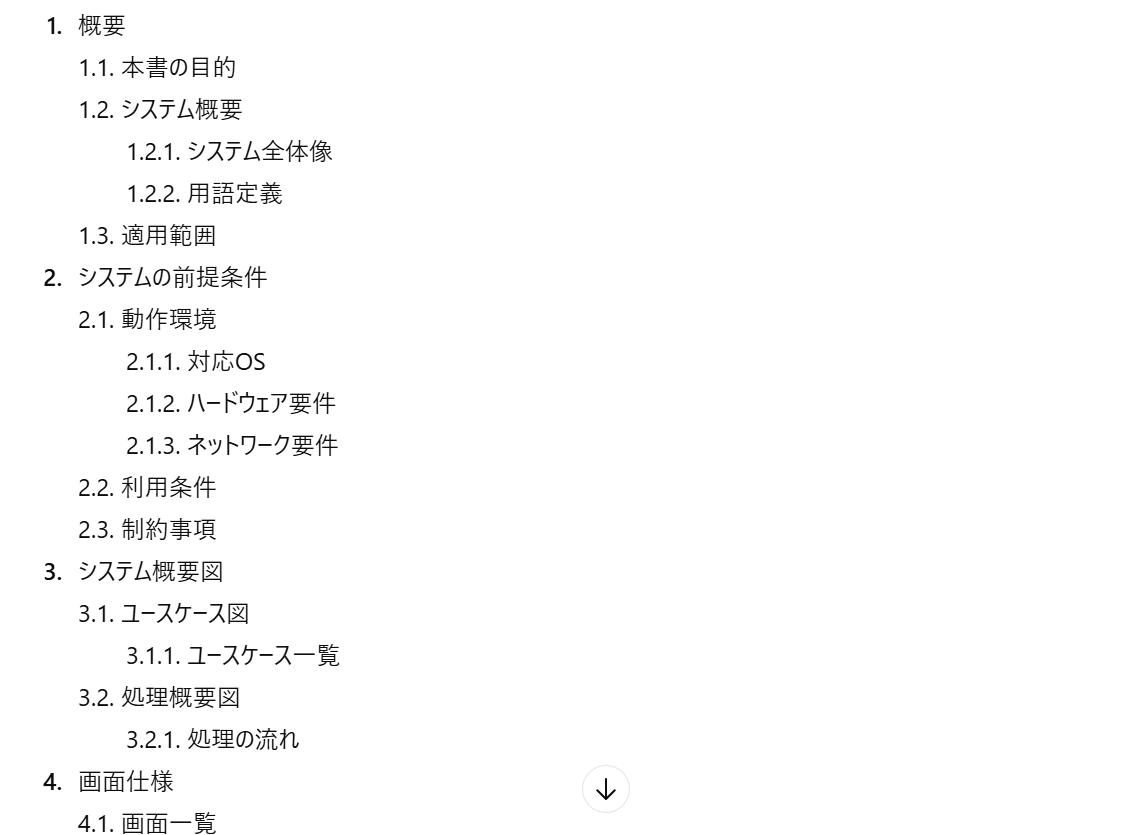
\includegraphics[width=0.8\textwidth]{images/正しい出力.png}
  }
  \captionof{figure}{出力形式指定ありの出力指示での出力例の一部}
  \label{fig:output_instruction_correct}
\end{figure}



\begin{figure}[tp]
\begin{tcolorbox}[
  colback=white,
  colframe=blue,
  fonttitle=\bfseries,
]
\footnotesize
\ttfamily
\fontsize{10}{11}\selectfont
\begin{verbatim}
【出力指示】
・上記情報に基づき、開発するシステムのシステム仕様書に必要な章立てを出力してください。
・ここでいう章立ては、以下の内容を含みます。
　・章と節、章タイトル、節タイトル、項、項タイトル
・章の追加や削除、順序の変更は自由に行って構いません。
・人間が考慮し忘れるような章立ても考えるのがあなたの役目です。考慮漏れが無いように、網羅性を高めてください。
\end{verbatim}
\end{tcolorbox}
\par\vspace{-20pt}
\captionof{figure}{図\ref{fig:output_instruction}から出力形式指定を削除した出力指示}
\label{fig:no_format}
\end{figure}

\begin{figure}[tp]
  \centering
  \fbox{
  \includegraphics[width=0.8\textwidth]{images/出力指示不適切な例.pdf}
  }
  \captionof{figure}{図\ref{fig:no_format}のプロンプトでの出力例の一部}
  \label{fig:output_instruction_no_format}
\end{figure}


\iffalse
本章では、図、表、数式の挿入方法について説明する。

% \section{図の挿入}

図を挿入するには、\verb|figure| 環境と \verb|\includegraphics| コマンドを使用する。

% \subsection{基本的な図の挿入}

図\ref{fig:example}に例を示す。

\begin{figure}[tp]
  \centering
  \includegraphics[width=0.5\linewidth]{./images/syokuji_computer.png}
  \caption{図の挿入例}
  \label{fig:example}
\end{figure}

上記の図は以下のコードで挿入できる：

\begin{verbatim}
\begin{figure}[tp]
  \centering
  \includegraphics[width=0.5\linewidth]{./images/syokuji_computer.png}
  \caption{図の挿入例}
  \label{fig:example}
\end{figure}
\end{verbatim}

% \subsection{画像ファイルの配置}

画像ファイルは \verb|images/| ディレクトリに配置する。
サポートされている画像形式：PNG、JPG、PDF など。

% \section{表の挿入}

表を挿入するには、\verb|table| 環境と \verb|tabular| 環境を使用する。

% \subsection{基本的な表の挿入}

表\ref{tb:example}に例を示す。

\begin{table}[tp]
  \caption{表の挿入例}
  \label{tb:example}
  \centering
  \begin{tabular}{|l|c|r|}
    \hline
    左寄せ & 中央寄せ & 右寄せ \\
    \hline
    データ1 & データ2 & データ3 \\
    データ4 & データ5 & データ6 \\
    \hline
  \end{tabular}
\end{table}

上記の表は以下のコードで挿入できる：

\begin{verbatim}
\begin{table}[tp]
  \caption{表の挿入例}
  \label{tb:example}
  \centering
  \begin{tabular}{|l|c|r|}
    \hline
    左寄せ & 中央寄せ & 右寄せ \\
    \hline
    データ1 & データ2 & データ3 \\
    データ4 & データ5 & データ6 \\
    \hline
  \end{tabular}
\end{table}
\end{verbatim}

% \section{数式の挿入}

% \subsection{インライン数式}

文中に数式を挿入する場合は、\verb|$...$| または \verb|\(...\)| を使用する。
例：$E = mc^2$ は有名な公式である。

% \subsection{ディスプレイ数式}

独立した行に数式を表示する場合は、\verb|equation| 環境を使用する。

\begin{equation}\label{eq:example}
  \int_0^\infty e^{-x^2} dx = \frac{\sqrt{\pi}}{2}
\end{equation}

式(\ref{eq:example})のように、数式にも番号とラベルを付けて参照できる。

% \subsection{複数行の数式}

複数行の数式を表示する場合は、\verb|align| 環境を使用する：

\begin{align}
  a + b &= c \\
  x + y &= z
\end{align}

% \section{図表の参照}

図や表を参照するには、\verb|\ref{}| コマンドを使用する：

\begin{itemize}
  \item 図\ref{fig:example}のように図を参照
  \item 表\ref{tb:example}のように表を参照
  \item 式(\ref{eq:example})のように数式を参照
\end{itemize}
\fi